\subsection{Etherless-cli}
\subsubsection{Struttura}
Il compito del modulo etherless-cli è quello di mettere a disposizione agli utenti finali dei comandi per interagire con la piattaforma \textit{Etherless}. Per permettere ciò abbiamo sviluppato le seguenti classi:
\begin{itemize}
	\item \textbf{Command}: classe astratta che si occupa di definire l'interfaccia necessaria per rappresentare correttamente un comando messo a disposizione dalla CLI;
	\item \textbf{CommandManager}: classe che si occupa di gestire i comandi. Permette la corretta interazione tra le classi derivate da Command e la libreria Yargs;
	\item \textbf{UserSession}: interfaccia che fornisce i metodi necessari per la gestione di una sessione utente; 
	\item \textbf{EthereumUserSession}: implementazione dell'interfaccia UserSession, in particolare si occupa di gestire sessioni utente in ambiente Ethereum; 
	\item \textbf{EtherlessContract}: interfaccia usata per definire le funzionalità che devono essere fornite dal modulo \textit{etherless-smart}; 
	\item \textbf{EthereumContract}: classe che implementa l'interfaccia EtherlessContract. Si occupa di interagire direttamente con il modulo \textit{etherless-smart} e con la blockchain Ethereum; 
	\item \textbf{FileManager}: interfaccia che permette di definire alcuni metodi fondamentali per la gestione di file; 
	\item \textbf{IPFSFileManager}: classe che implementa l'interfaccia FileManager, permette di salvare e recuperare file tramite il protocollo IPFS; 
	\item \textbf{FileParser}: interfaccia che permette di definire i metodi necessari per eseguire il processo di parsing di file sorgente; 
	\item \textbf{JSFileParser}: classe che implementa l'interfaccia FileParser, si occupa di gestire il parsing di file scritti in JavaScript; 
	\item \textbf{EtherlessManager}: classe che si occupa di eseguire controlli ed interagire con le altre classi per fornire le funzionalità che sono richieste dai comandi. 
\end{itemize}

\subsubsection{Design}
Il modulo etherless-cli è stato progettato avendo come obiettivo principale l'estendibilità, in particolare abbiamo voluto garantire la possibilità di integrare nuove funzionalità senza apportare modifiche sostanziali alla struttura esistente. A tale scopo sono state prese le seguenti scelte progettuali: 
\begin{itemize}
	\item è stata definita la classe astratta Command: in questo modo è possibile andare ad introdurre nuovi comandi semplicemente estendendo tale classe;  
	\item è stata definita l'interfaccia FileManager, che permette di definire diverse implementazioni che usano protocolli per la gestione di file diversi; 
	\item è stata definita l'interfaccia FileParser, che consente all'applicativo di gestire il parsing di file sorgenti senza essere vincolati ad un unico linguaggio di programmazione; 
	\item è stata definita l'interfaccia EtherlessContract, che permette di definire le funzionalità che devono essere fornite dal modulo etherless-smart, senza essere vincolati alla sua interfaccia pubblica; 
	\item è stata definita l'interfaccia UserSession, che permette di definire le funzionalità caratteristiche di una sessione utente in maniera indipendente dalle librerie utilizzate per la memorizzazione dei dati ad essa associati.  
\end{itemize}

Durante la progettazione abbiamo fatto riferimento principalmente ai seguenti design pattern:
\begin{itemize}
	\item \textbf{Command}: come design pattern comportamentale per la gestione dei comandi messi a disposizione della CLI. In particolare è stata definita una classe astratta Command che viene estesa da ogni comando. Sfruttando tale design pattern la classe CommandManager è in grado di gestire richieste di cui non conosce i particolari; 

	\item \textbf{Facade}: come design pattern strutturale per lo sviluppo della classe EtherlessManager, che si occupa di eseguire vari controlli ed interagire con le opportune classi per gestire le richieste eseguite dai comandi;

	\item \textbf{Constructor injection}: come design pattern architetturale per lo sviluppo della classe EtherlessManager. Tutte le dipendenze vengono dichiarate come parametri del costruttore: in questo modo la classe non si deve occupare della creazione degli oggetti considerati ma solo del loro utilizzo. 
\end{itemize}

\subsubsection{Diagramma dei package}

\begin{landscape}
	\centerline{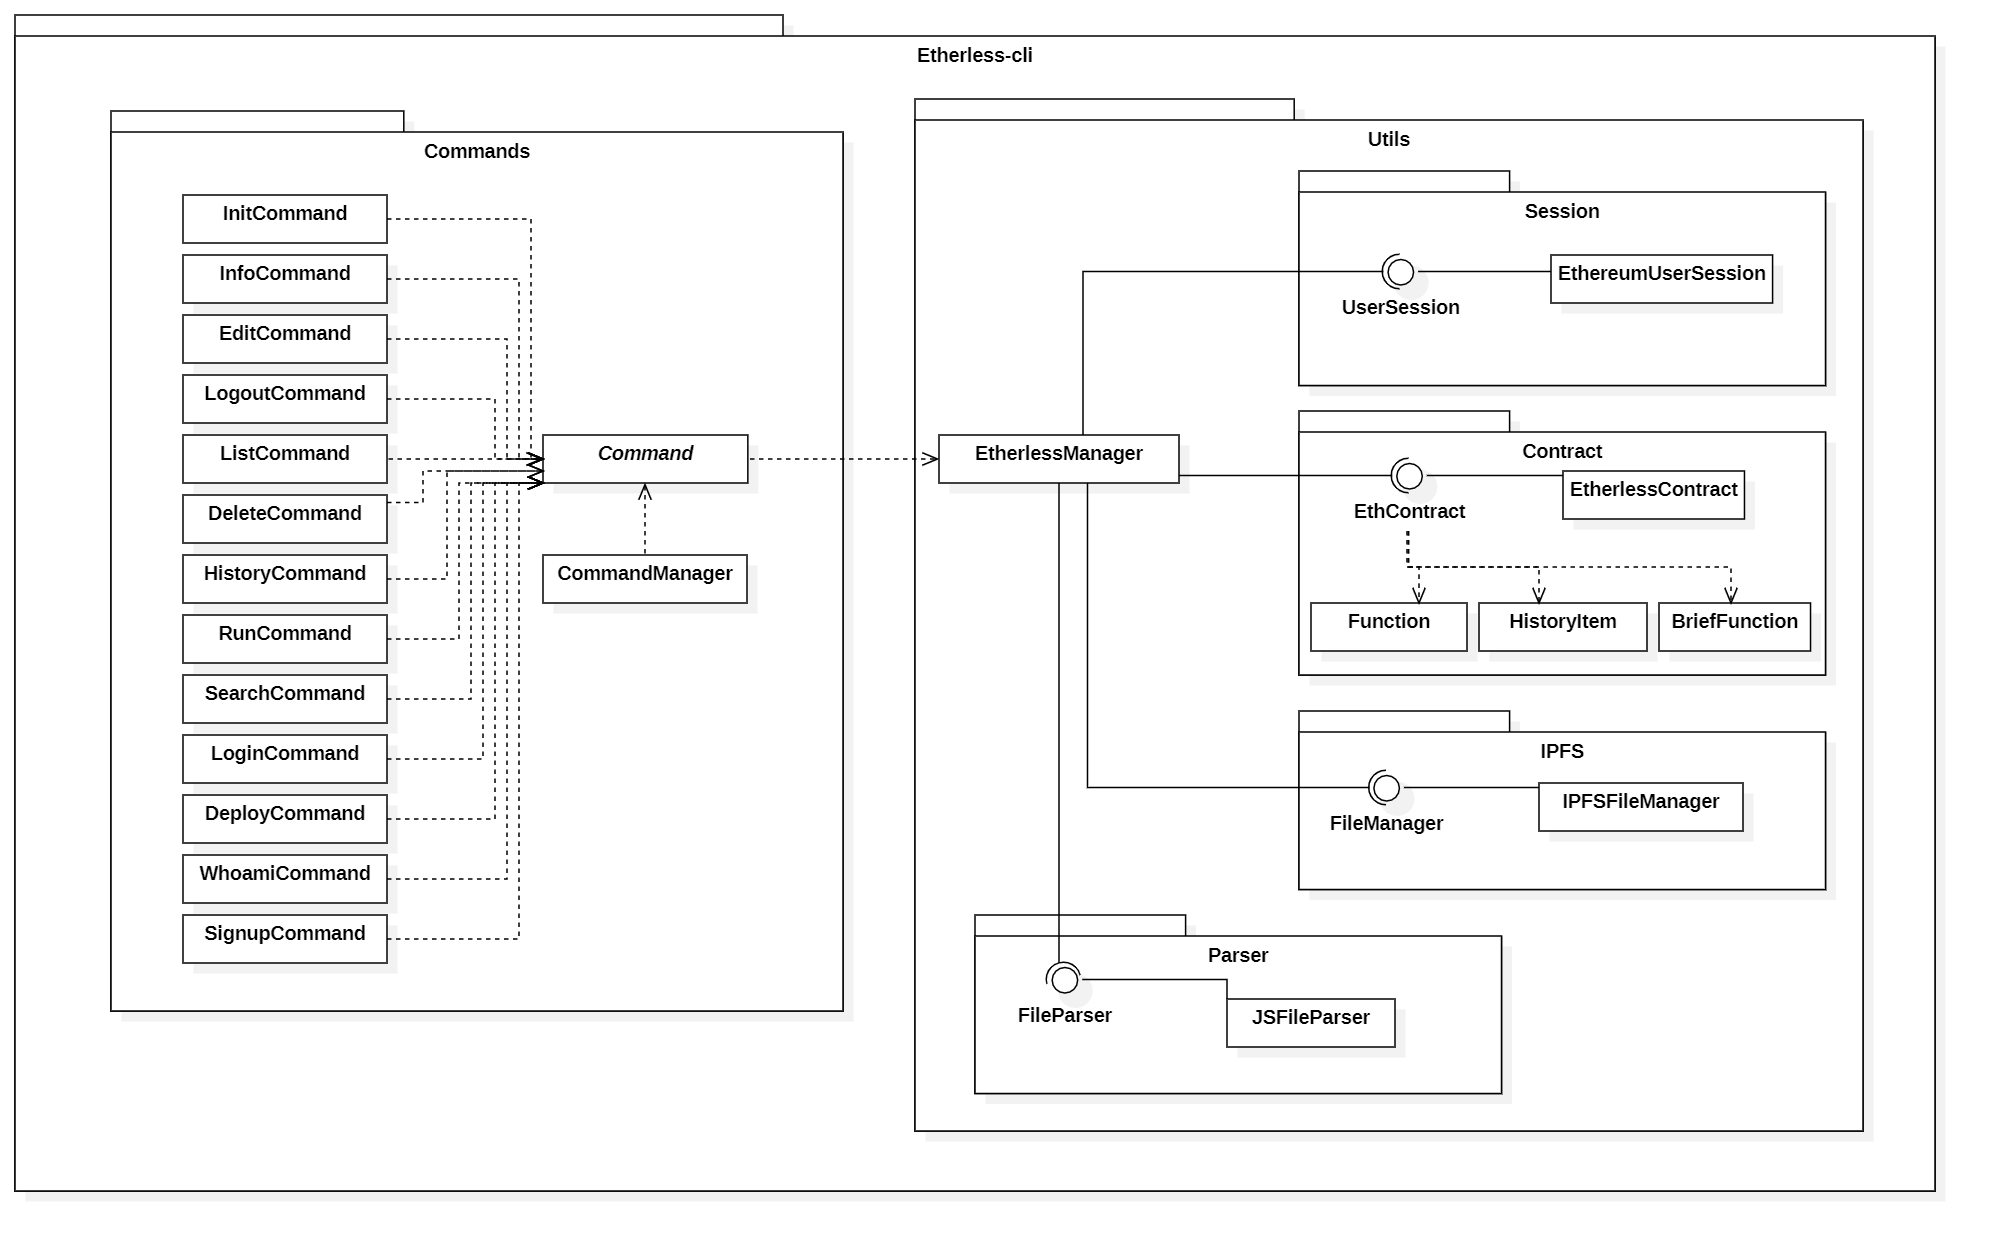
\includegraphics[scale=0.33]{diagrammi/etherless-cli/package.png}}
\end{landscape}

\centerline{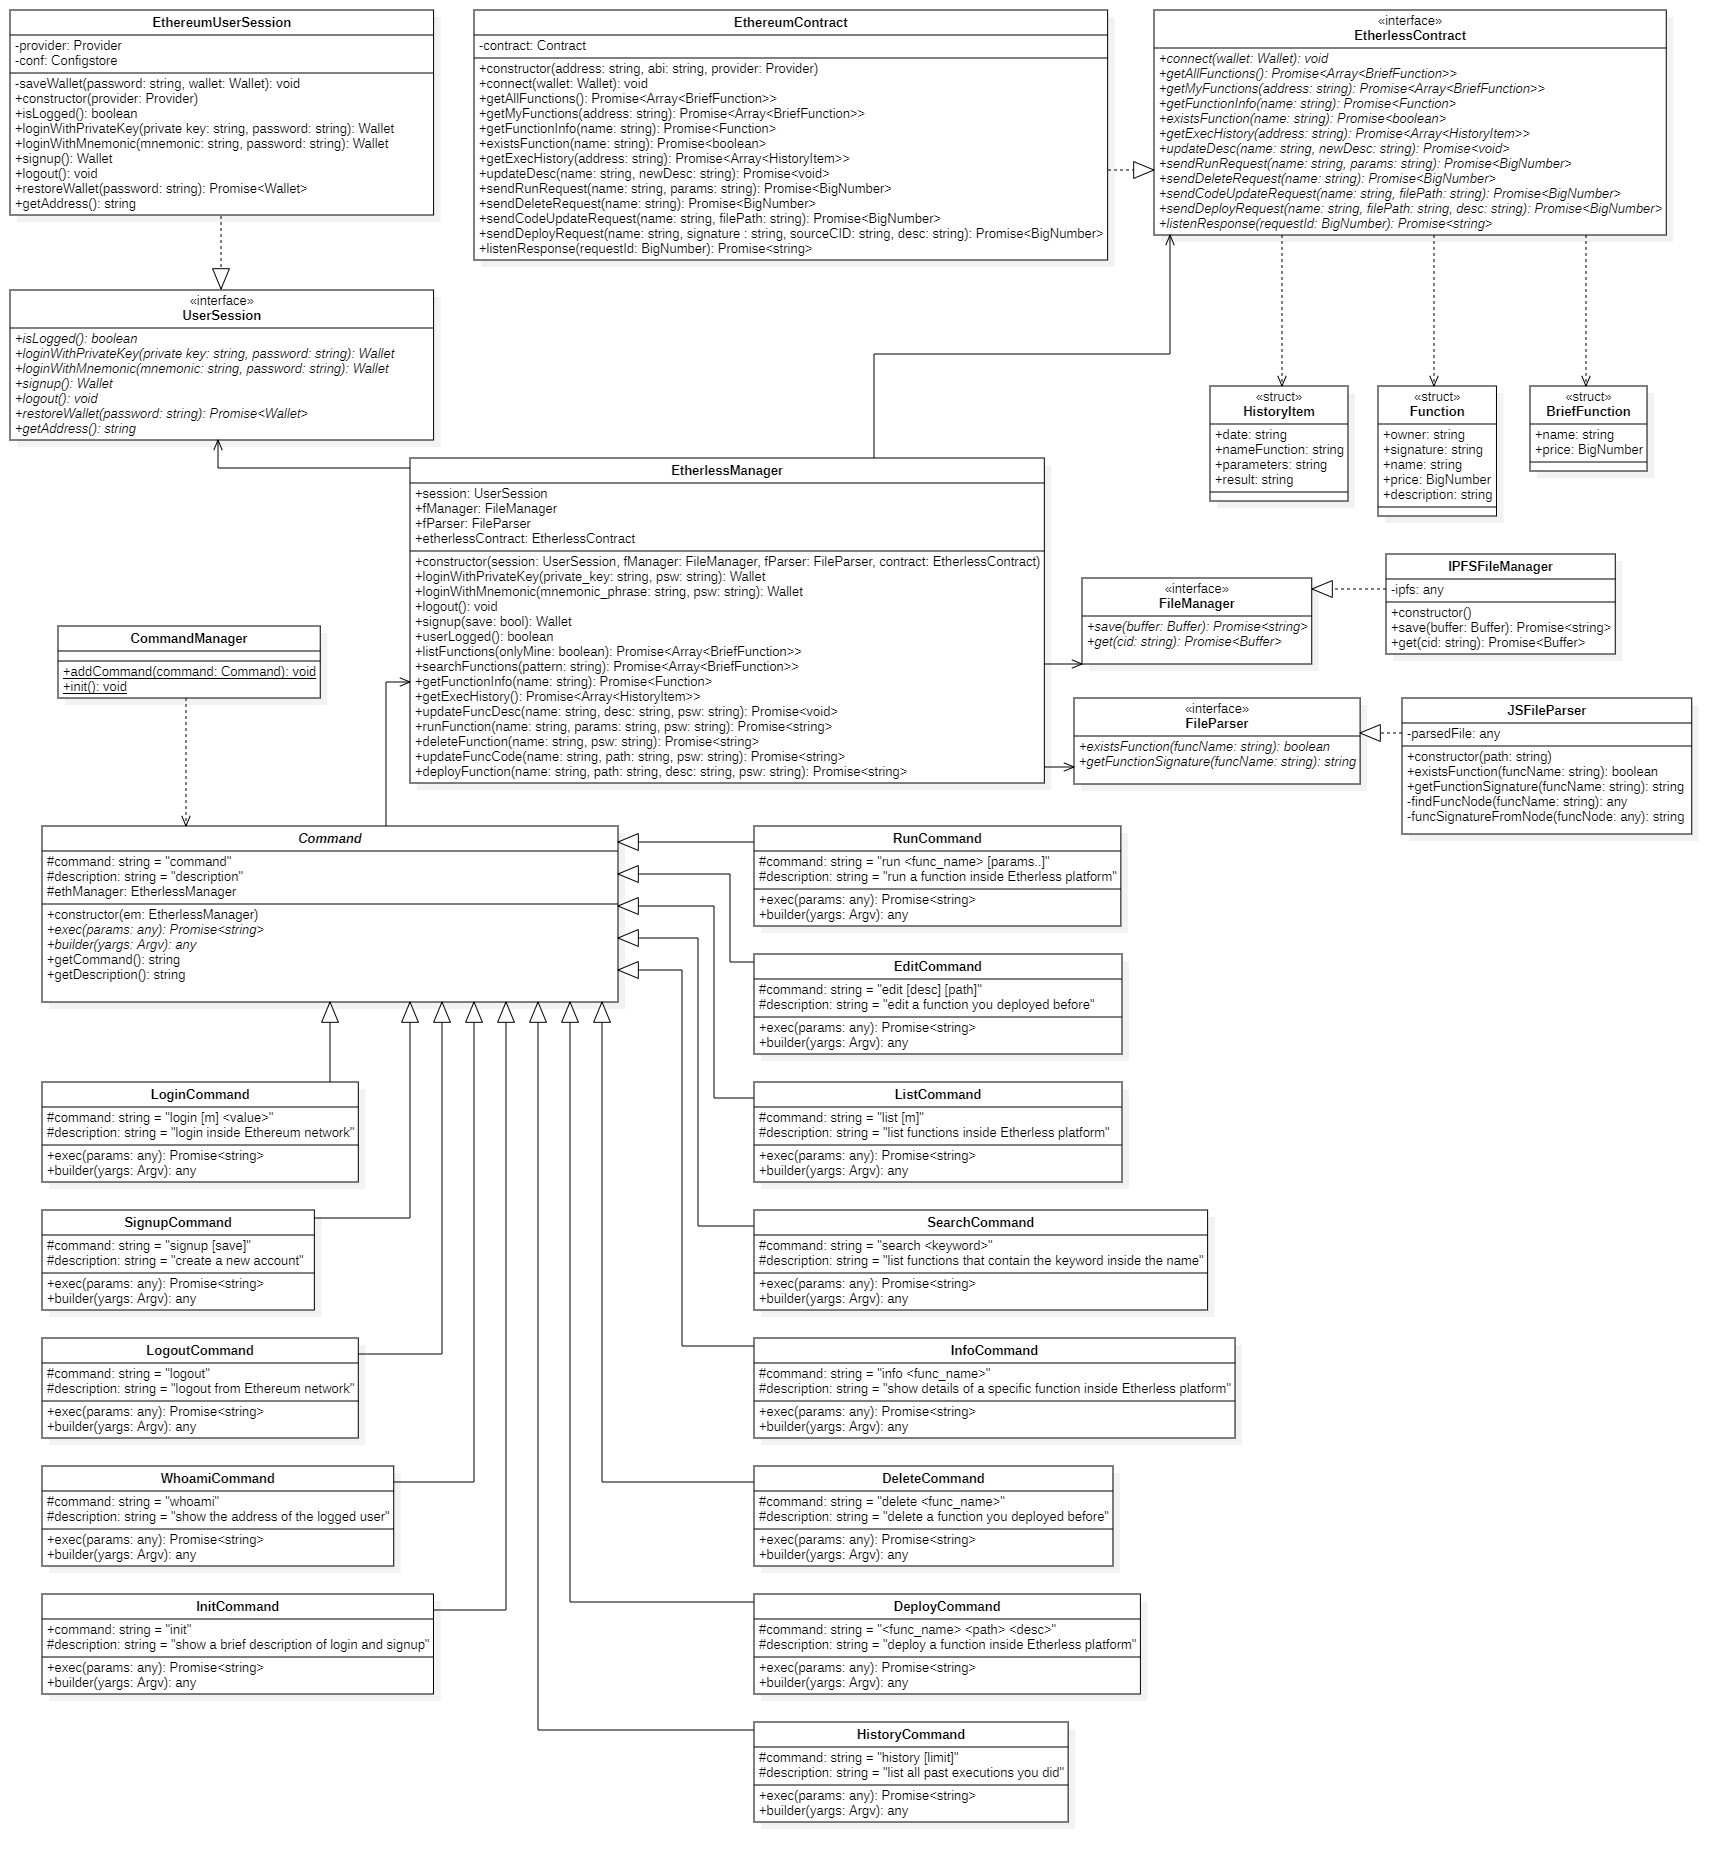
\includegraphics[height=19cm, width=16cm]{diagrammi/etherless-cli/classi.png}}

\subsubsection{Diagrammi di sequenza}
\begin{figure}[H]
	\noindent
	\makebox[\textwidth]{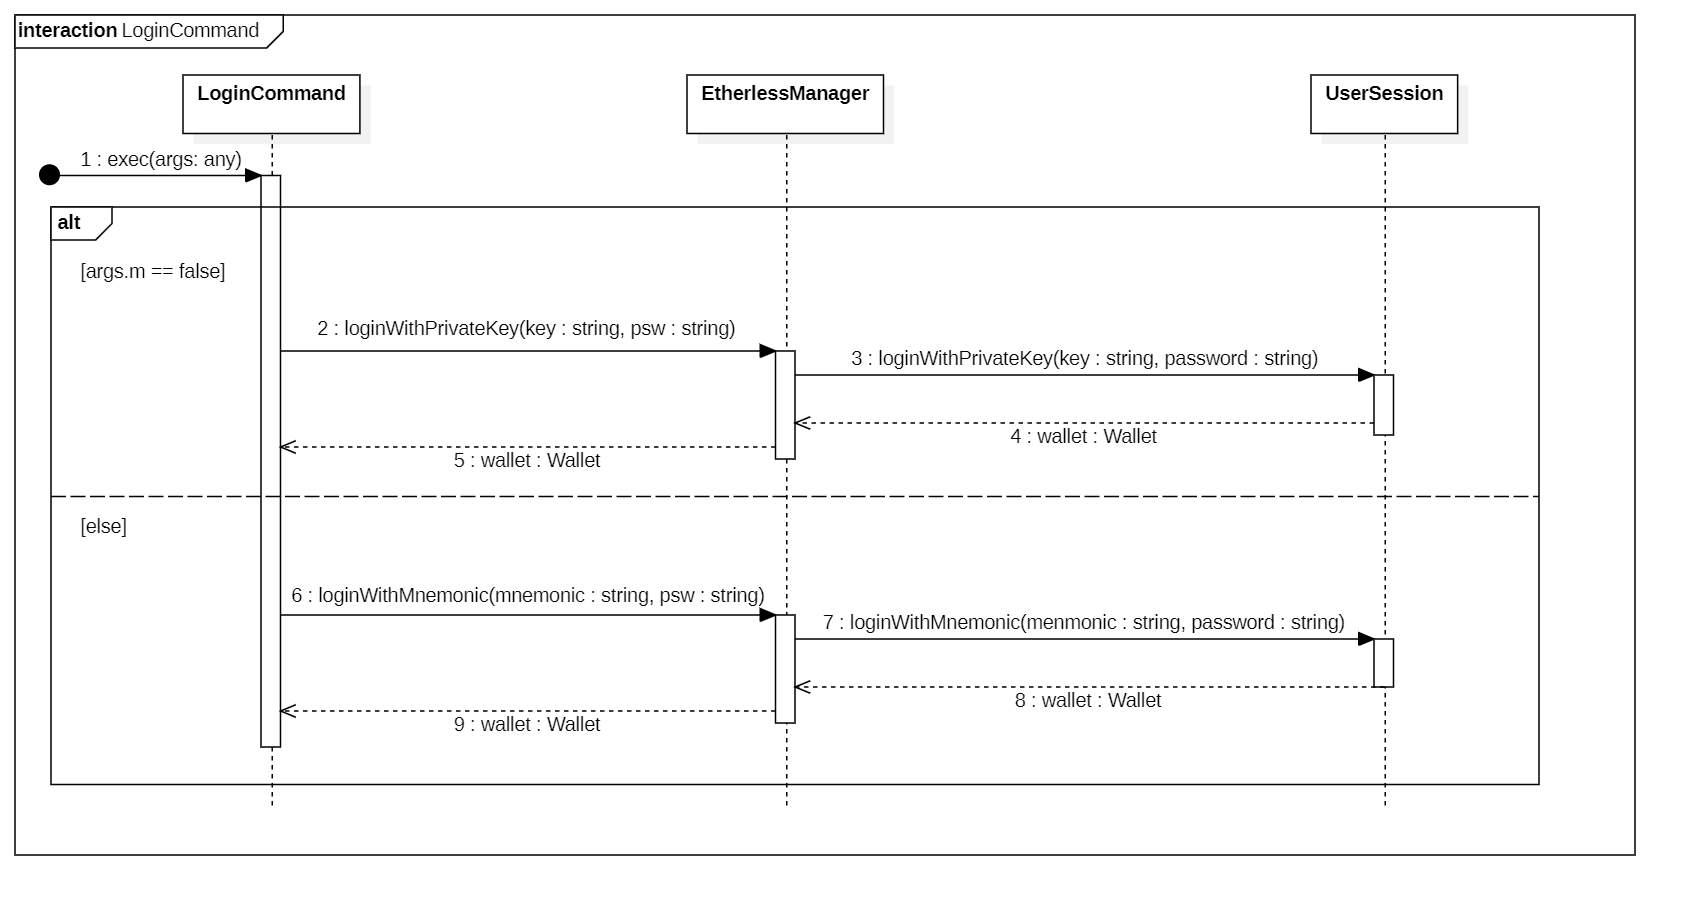
\includegraphics[scale=0.25]{././diagrammi/etherless-cli/loginCommand.png}}
	\caption{Diagramma di sequenza della procedura di autenticazione.}
\end{figure}
\begin{figure}[H]
	\noindent
	\makebox[\textwidth]{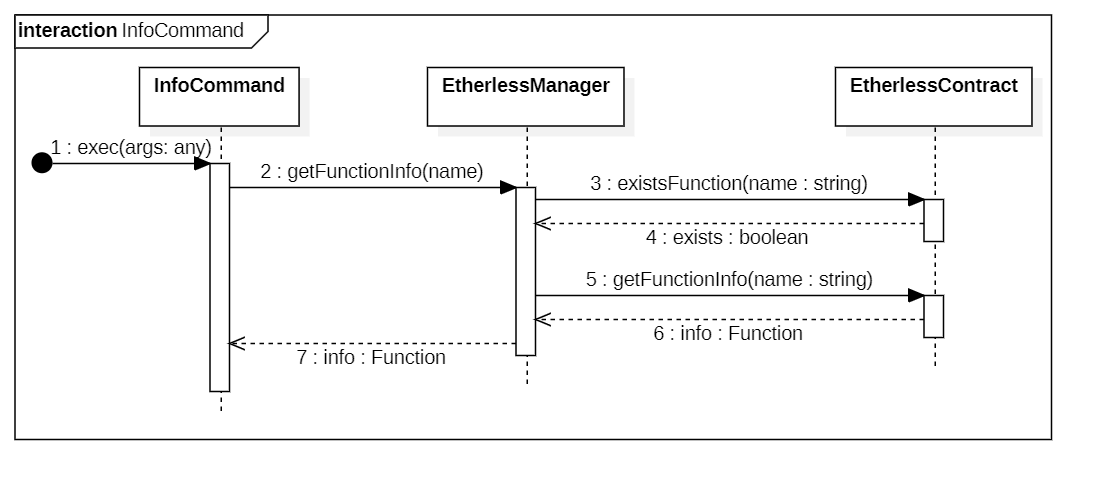
\includegraphics[scale=0.25]{././diagrammi/etherless-cli/infoCommand.png}}
	\caption{Diagramma di sequenza per le informazioni dettagliate di una funzione.}
\end{figure}
\begin{figure}[H]
	\noindent
	\makebox[\textwidth]{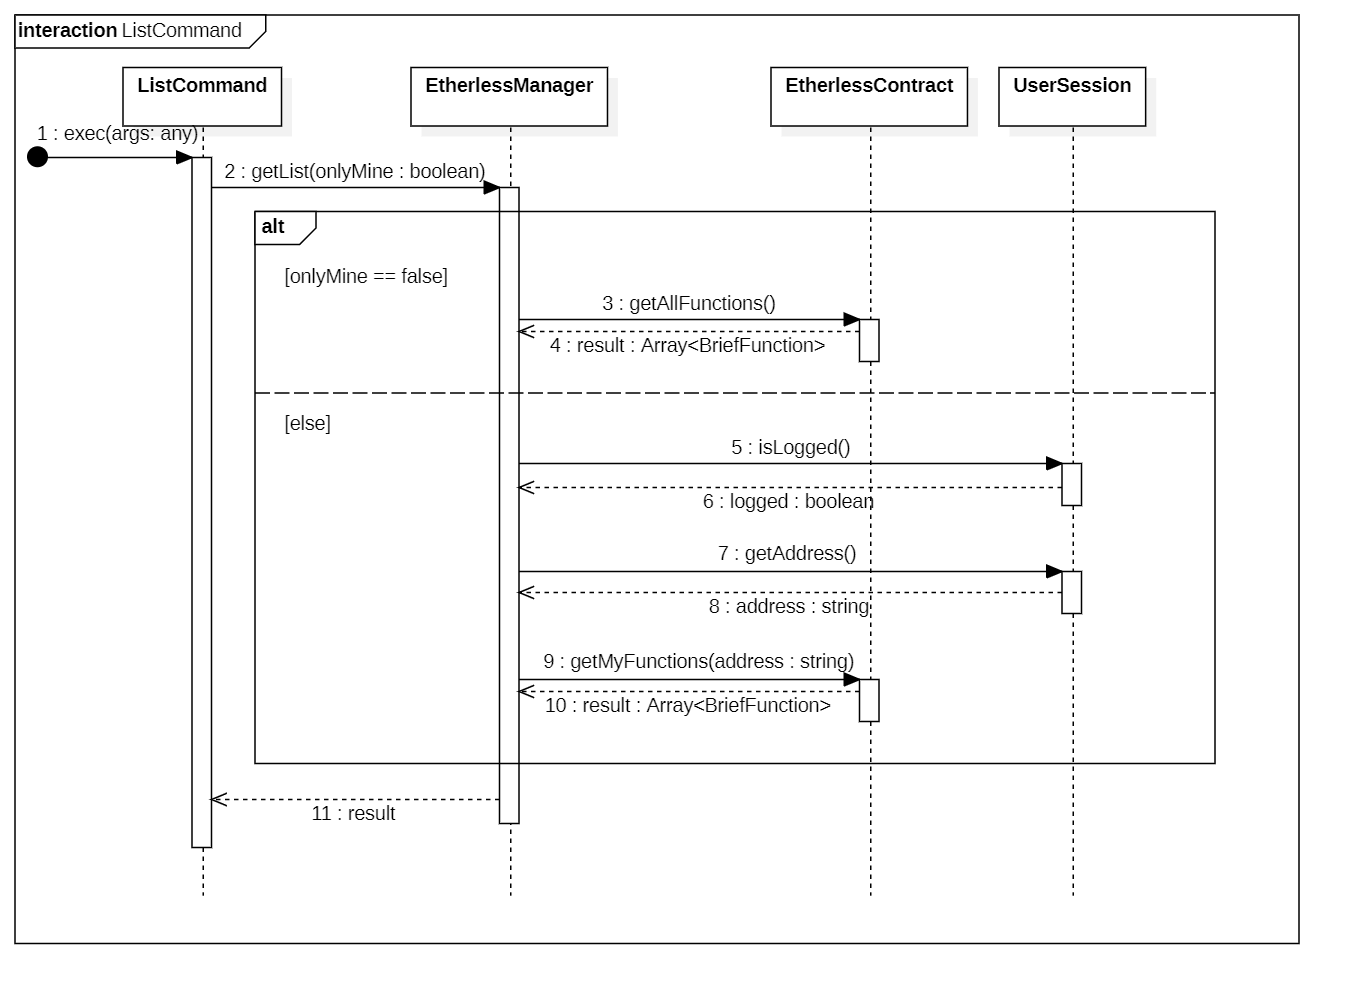
\includegraphics[scale=0.2]{././diagrammi/etherless-cli/listCommand.png}}
	\caption{Diagramma di sequenza per la lista delle funzioni disponibili.}
\end{figure}
\begin{figure}[H]
	\noindent
	\makebox[\textwidth]{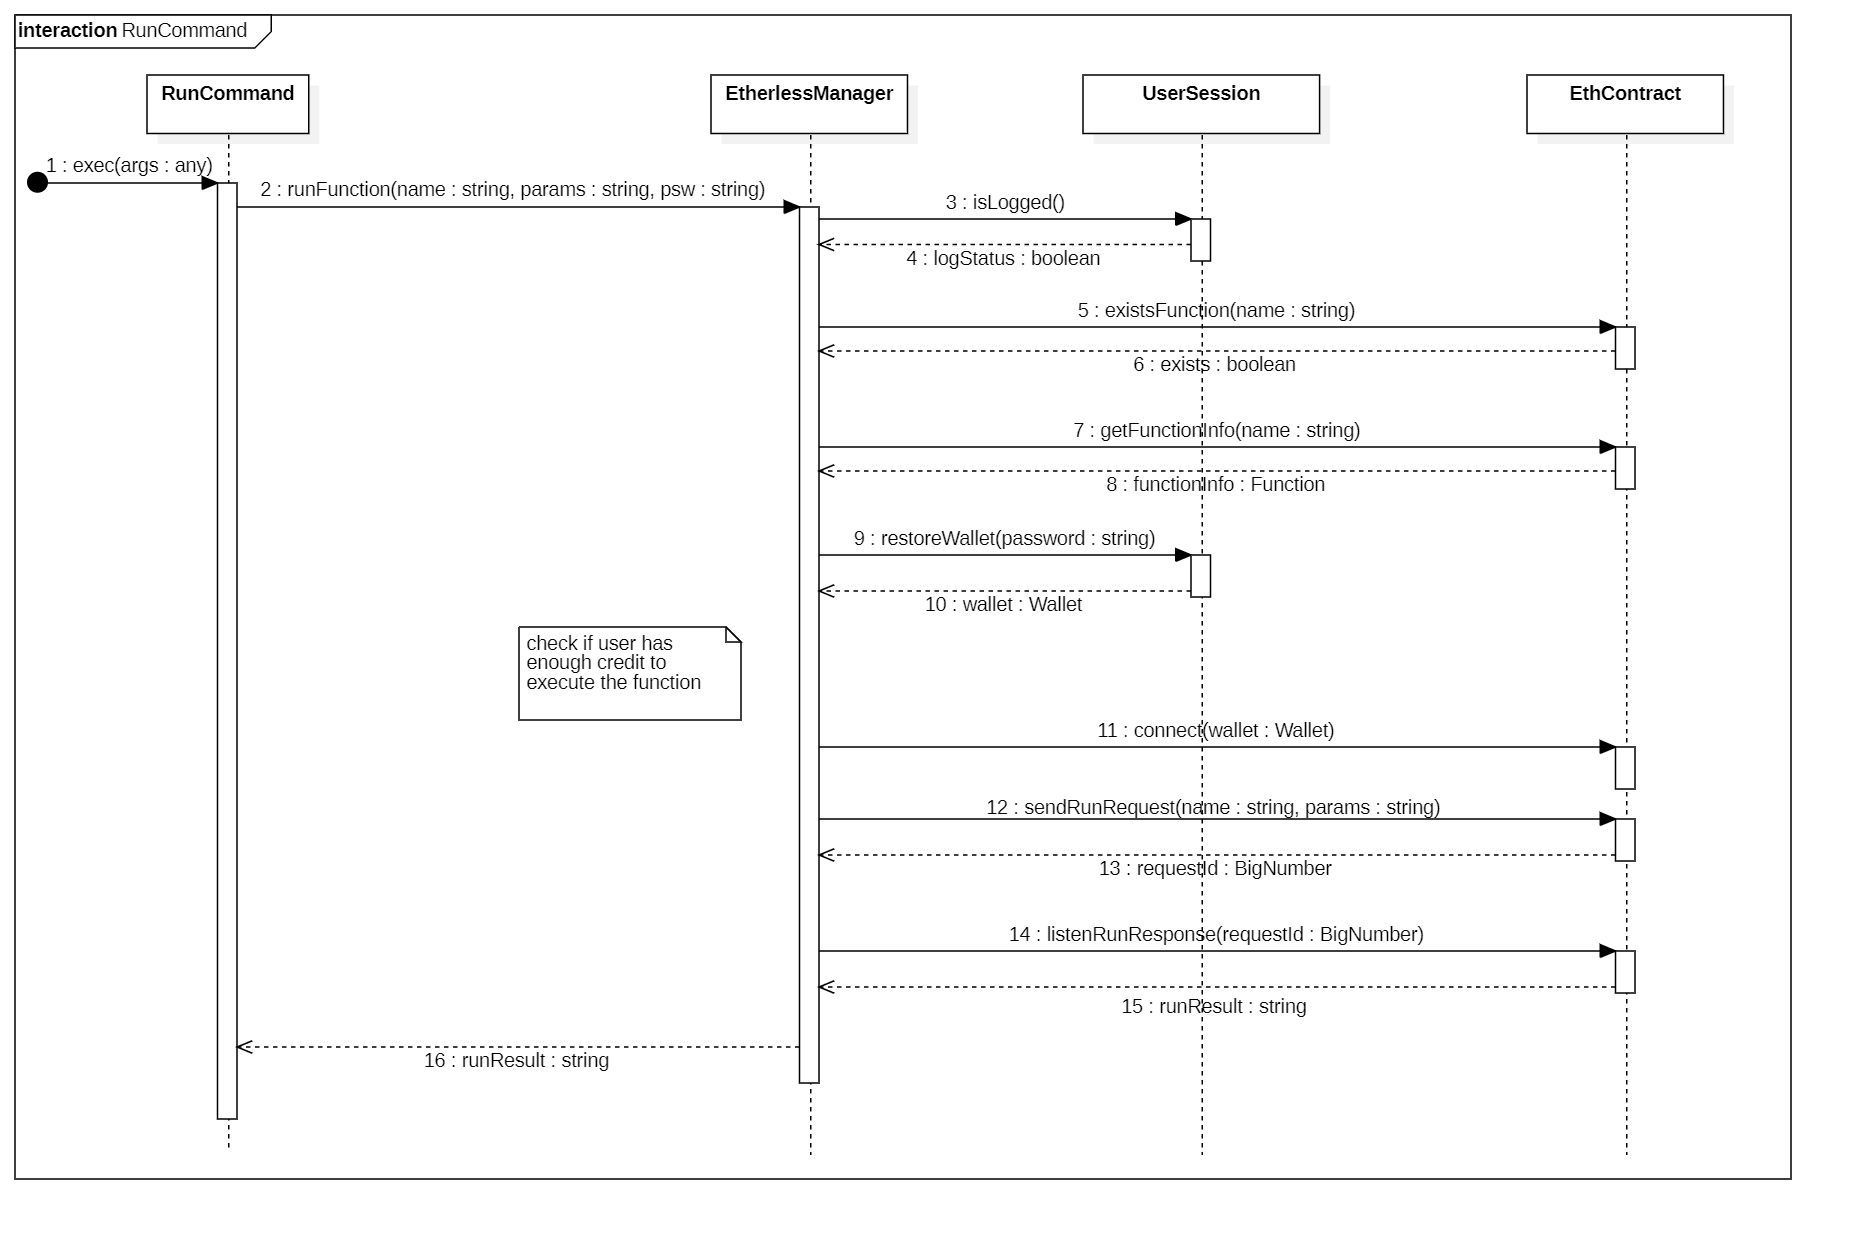
\includegraphics[scale=0.2]{././diagrammi/etherless-cli/runCommand.png}}
	\caption{Diagramma di sequenza dell'esecuzione di una funzione.}
\end{figure}
\begin{figure}[H]
	\noindent
	\makebox[\textwidth]{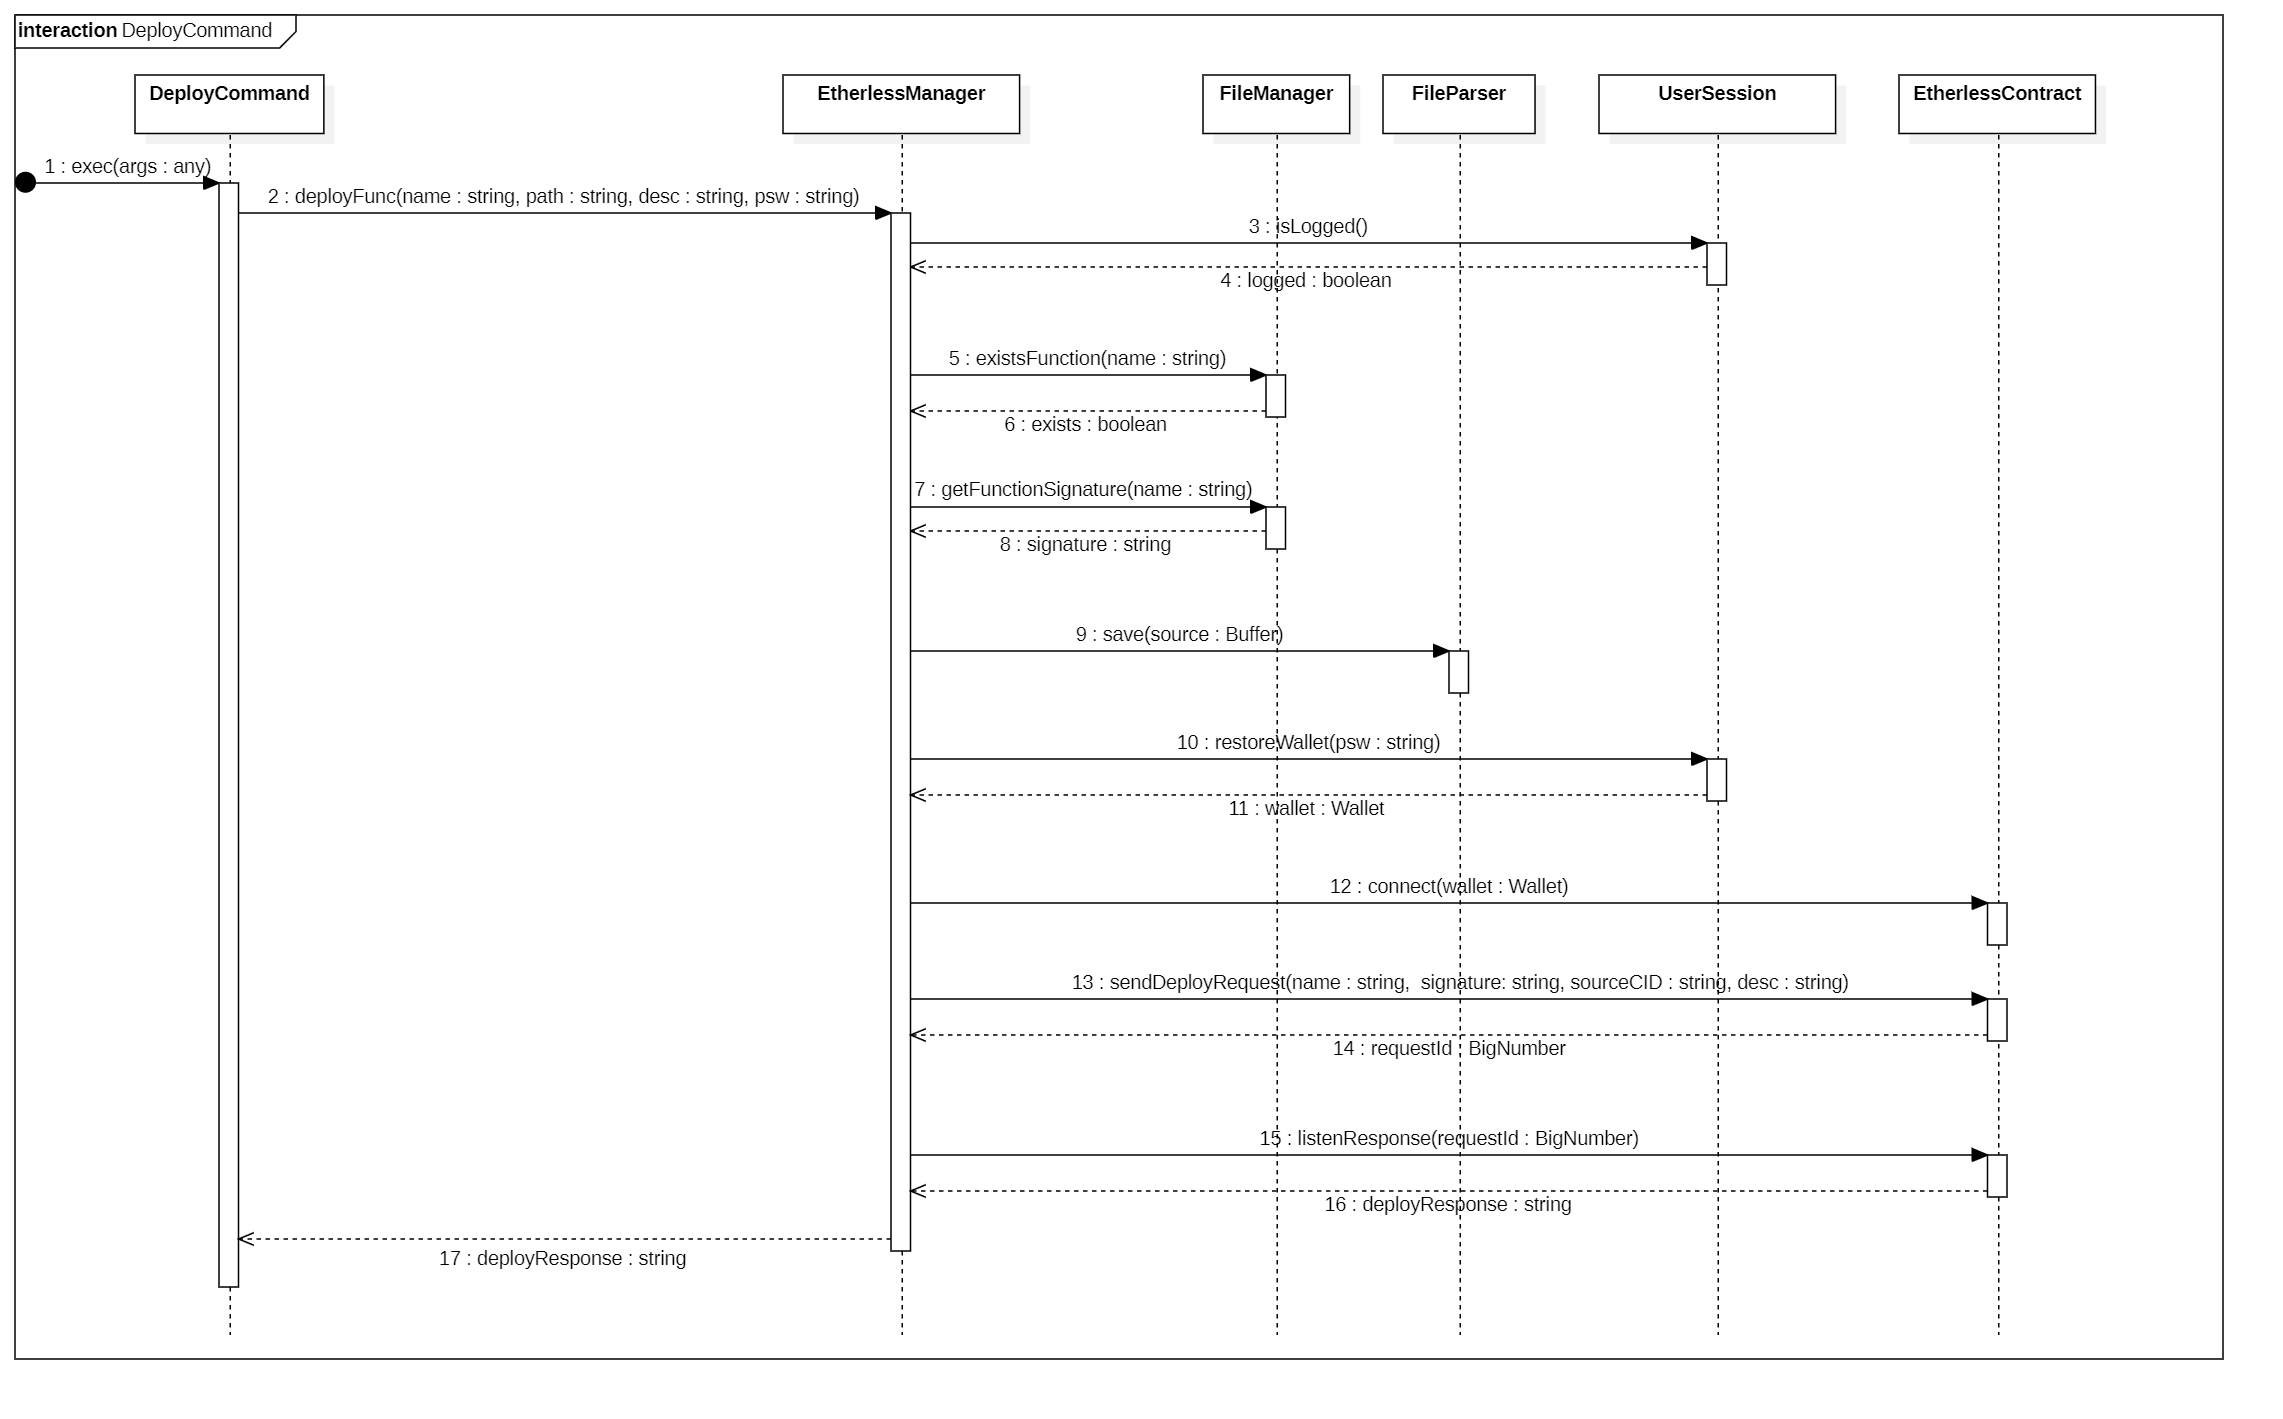
\includegraphics[scale=0.25]{././diagrammi/etherless-cli/deployCommand.png}}
	\caption{Diagramma di sequenza del deploy di una funzione.}
\end{figure}
\begin{figure}[H]
	\noindent
	\makebox[\textwidth]{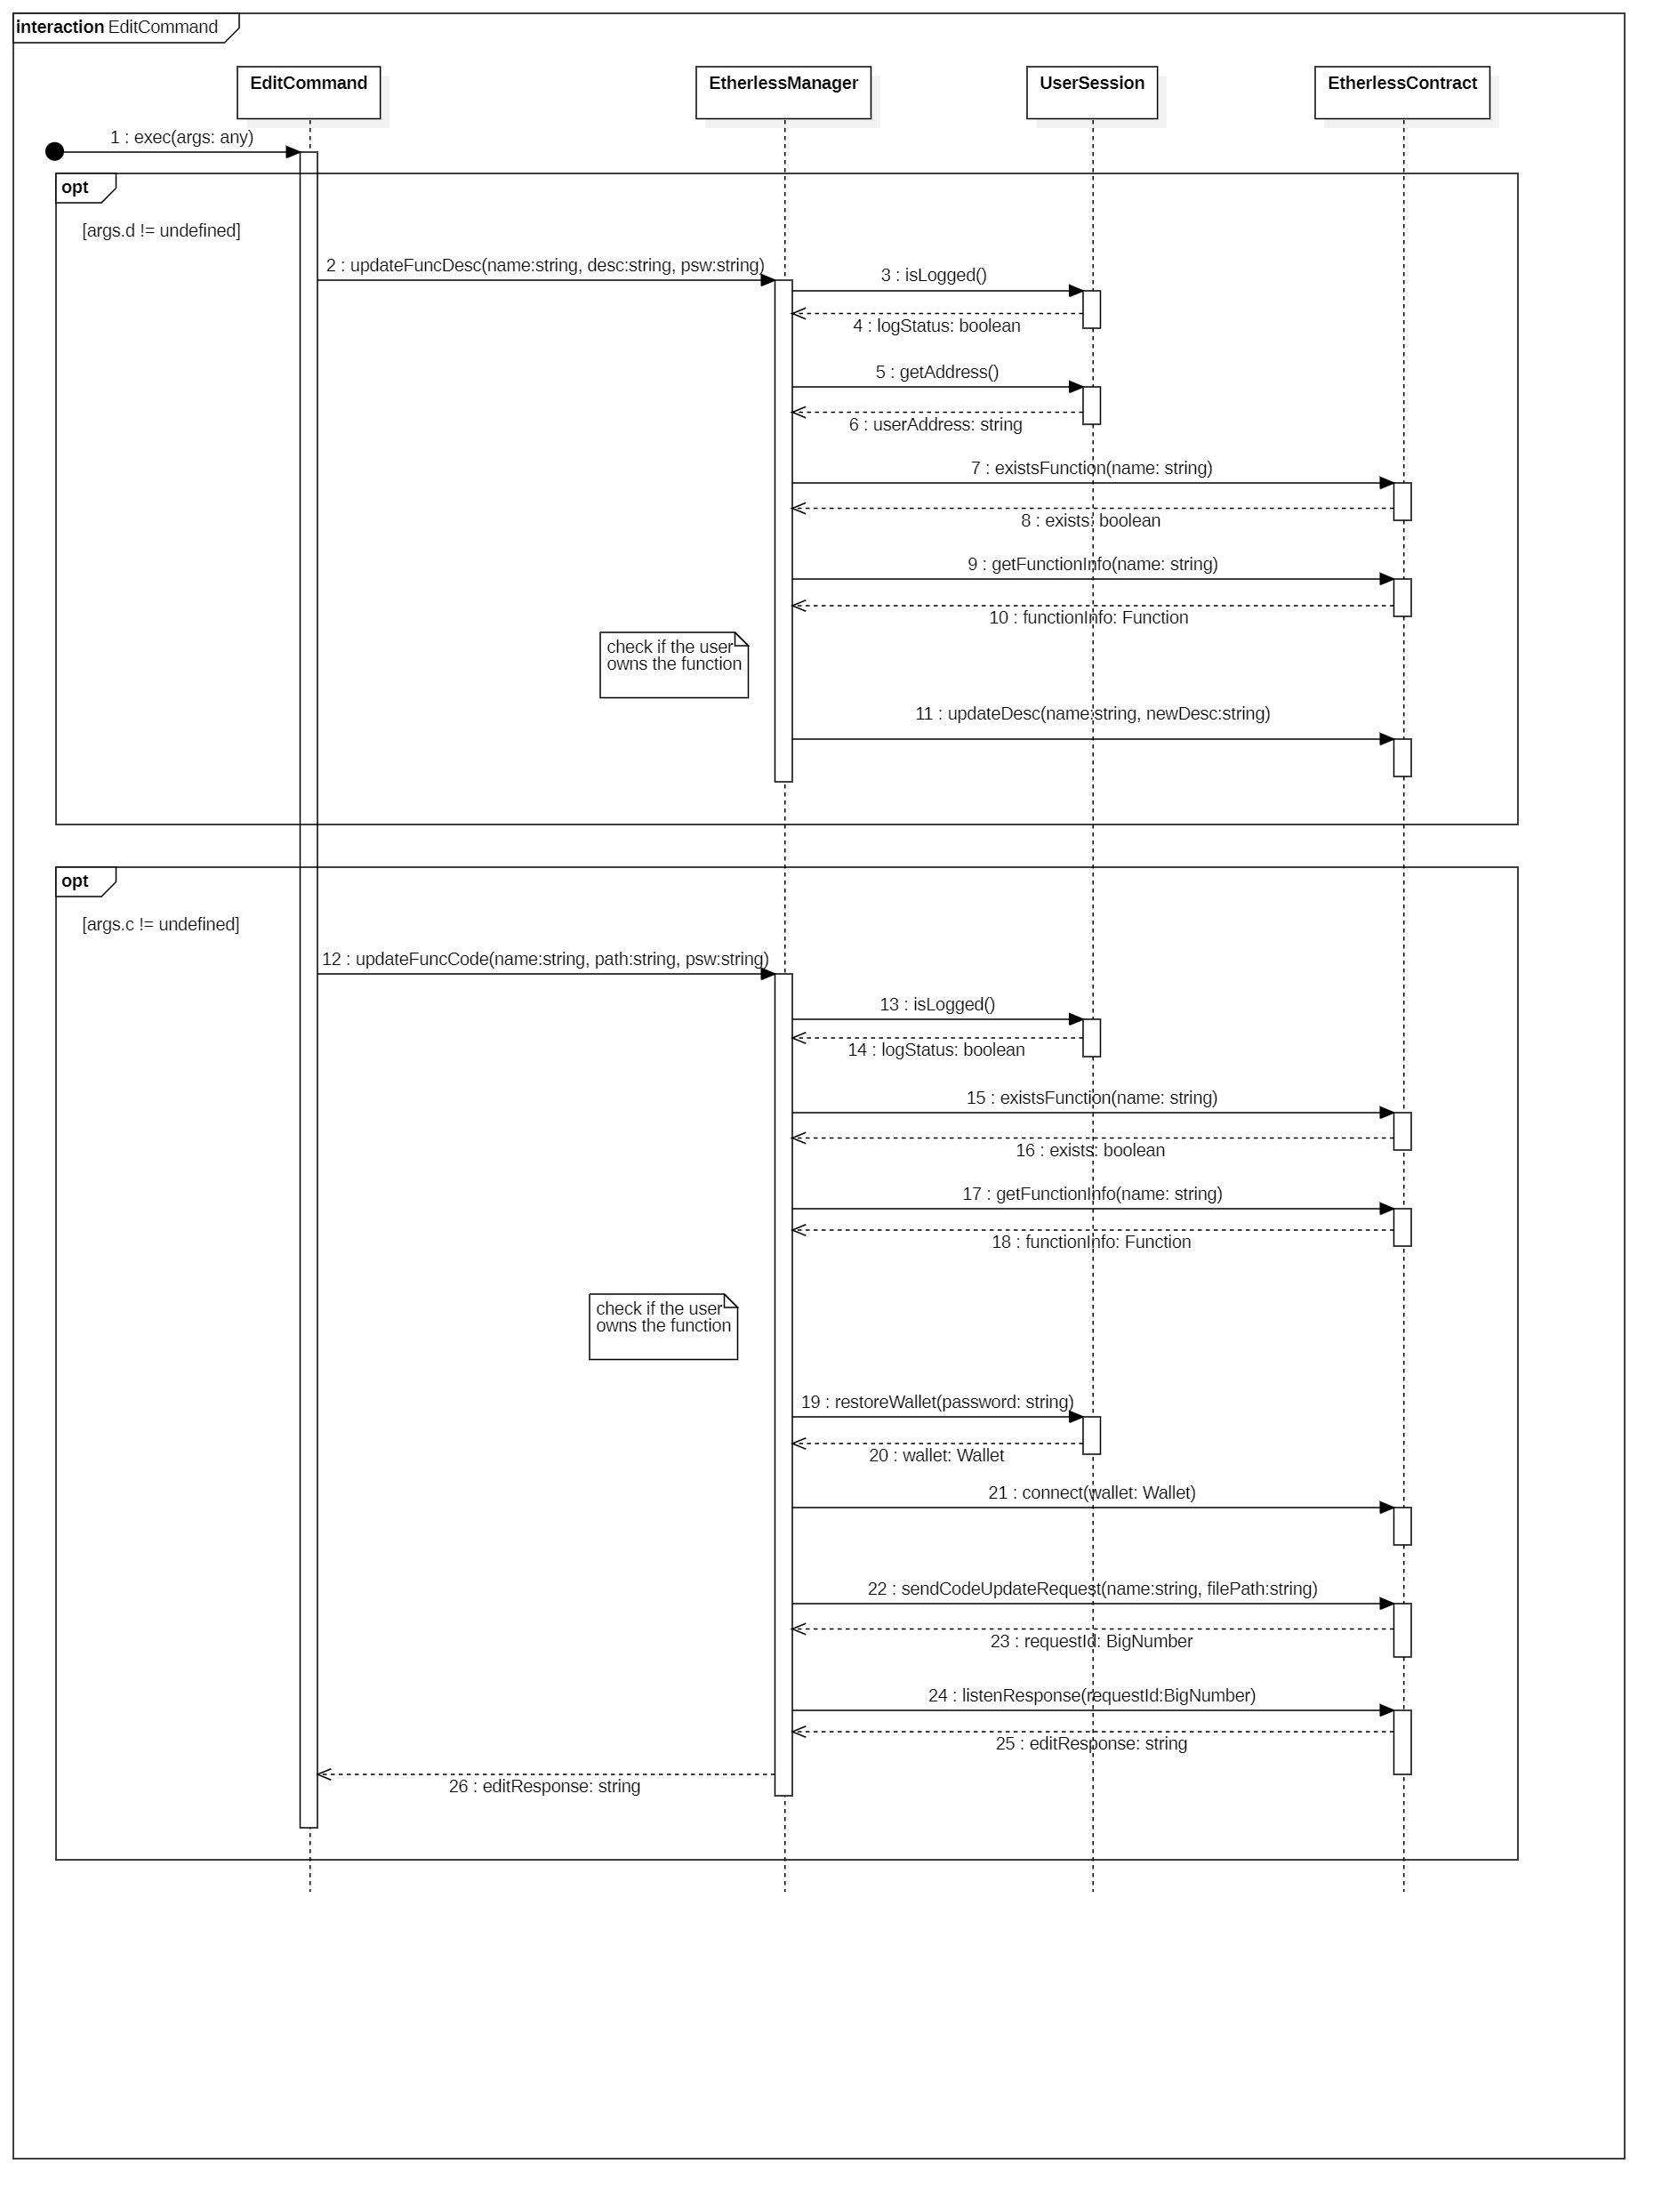
\includegraphics[scale=0.25]{././diagrammi/etherless-cli/editCommand.png}}
	\caption{Diagramma di sequenza della modifica di una funzione.}
\end{figure}

\begin{figure}[H]
	\noindent
	\makebox[\textwidth]{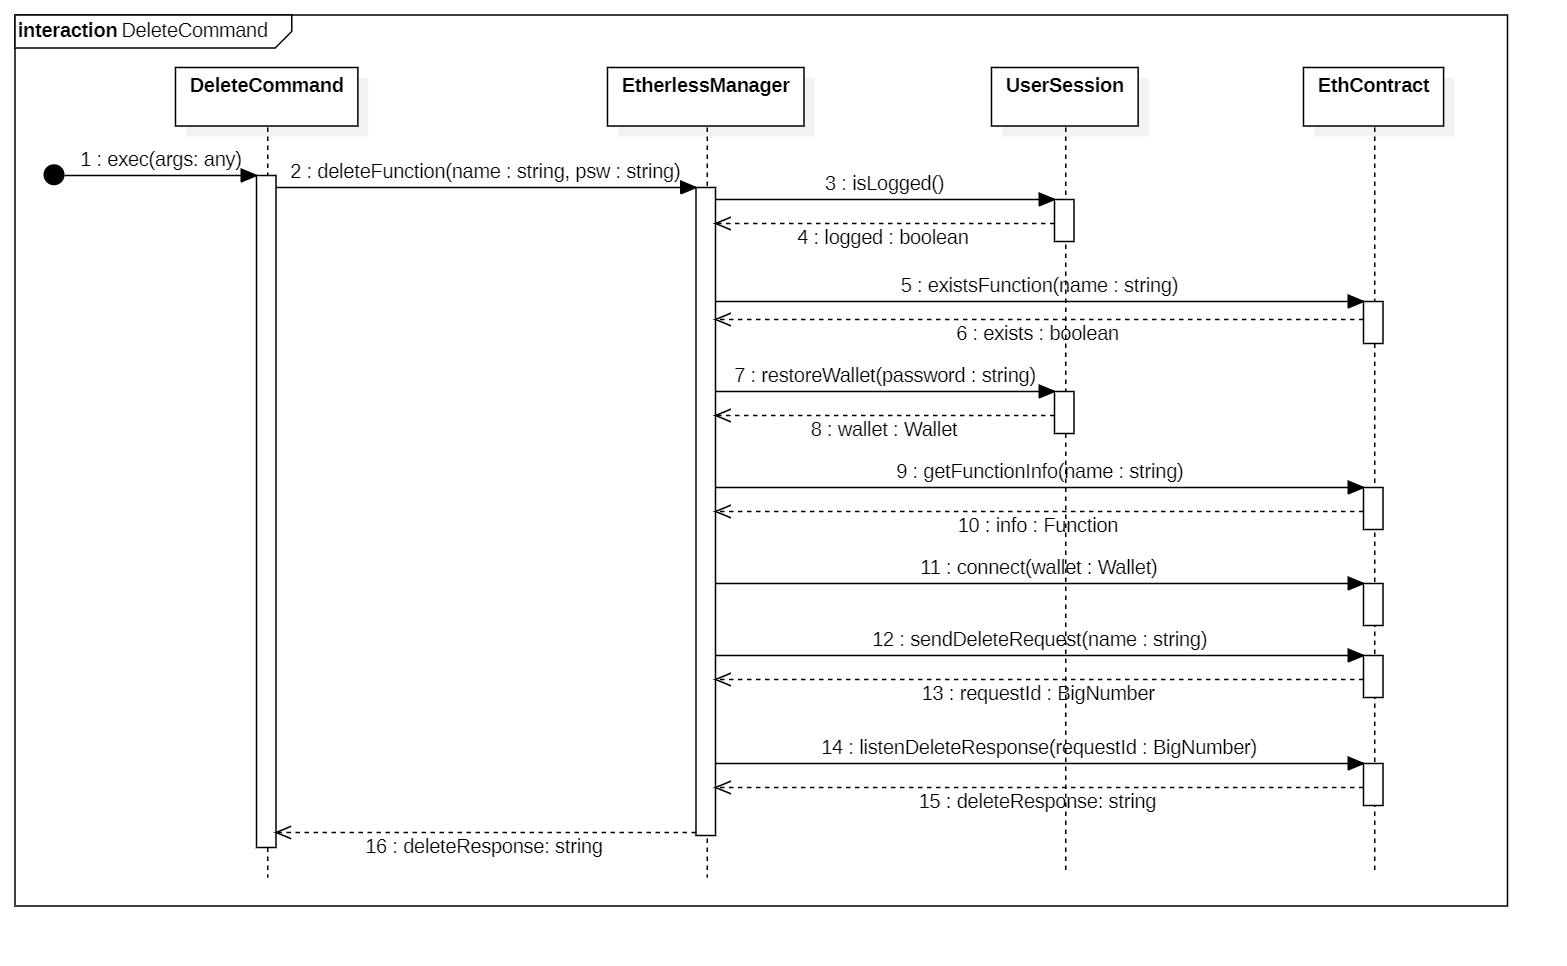
\includegraphics[scale=0.25]{././diagrammi/etherless-cli/deleteCommand.png}}
	\caption{Diagramma di sequenza dell'eliminazione di una funzione.}
\end{figure}


